% Chapter 5
\chapter{Evaluation}\label{ch:eval}
To evaluate the proposed method two classes of experiments are carried out. In a first step an example planner is implemented which mimics the local planning step and provides an easy way to test the trajectory evaluation separated from the rest of a conventional planning system.

With the gained data the algorithms are improved and used to extend existing local planner. A fully simulated environment and robotic model using a sophisticated physic engine together with a complete robot navigation system is used to compare the original implementation of the local planner with our approach.
 
\section{Experiments with Sample Planner}
The trajectory sampling and selection of a common DWA approach are implemented in python minimizing a simpler cost function $f_c(v,w)$ (cf. Equation~\ref{eq:simplecost}), where $f_g(v,w)$ is the distance of the center of the robot in the end position to a predefined goal position, and $f_o(v,w)$ is the maximal distance to an obstacle on the trajectory path.

\begin{equation}
   f_c(v,w)=\alpha f_g(v,w) - \beta f_o(v,w)
   \label{eq:simplecost}
\end{equation}

To select a benchmark cost a brute force search is performed on random generated test instances, evaluating a fixed number of trajectories. 
The time the algorithm needs to find this benchmark solution is used to compare their performance.

All algorithm are tested using different minimal, and maximal velocities to account for different acceleration limits. 

The weighting coefficients of the cost function are fixed to $\alpha=0.01$ and $\beta=1$. The local goal is also at a fixed location in the map. 
The step size of the collision test is fixed to 0.015 meter. 
Forward simulation time is fixed to one second. 

The following 60 test instances include different obstacle counts and random placement of quadratic obstacles:
\begin{itemize}
\item 15 instances with 1 obstacle and side length 1 meter.
\item 15 instances with 3 obstacles and side length 1 meter.
\item 15 instances with 5 obstacles and side length 0.5 meter.
\item 15 instances with 25 obstacles and side length 0.1 meter.
\end{itemize}

The instances simulate a snapshot of the local environment of the robot at a given time point, which is used as a local map for input of the local planner.
The resolution of the maps is fixed to 0.05 meter/pixel, resulting in a quadratic map of size 7.5 meter. Figure~\ref{fig:fig_instances} illustrates three random instances. 
%\begin{figure}[thpb]
\begin{figure}[thpb]
     \footnotesize
      \centering
      \myfloatalign
      \setlength\fboxsep{0pt}
      \setlength\fboxrule{0.5pt}
       \subfloat[]
       {  
           \fbox{
\includegraphics[width=0.3\textwidth]{figures/01_1_b_nocost.png}}
       } 
       \subfloat[]
       {  
           \fbox{
\includegraphics[width=0.3\textwidth]{figures/03_5_m_nocost.png}}
       } 
       \subfloat[]
       {  
           \fbox{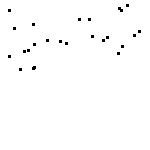
\includegraphics[width=0.3\textwidth]{figures/04_25_s_nocost.png}}
       }        
       \caption{Figures (a)-(c) show 3 out of 60 random instances for experiments. The instances differ in number and size of obstacles and are used for local costmap creation.}
      \label{fig:fig_instances}
   \end{figure}

The following list shows the tested algorithm:
\begin{itemize}
\item{\bf{Random Search with Tabu List:}} A repeated random guess of a velocity tuple $(v,w)$ (Random).
\item{\bf{Iterated Local Search:}} Performing Iterated Local Search with 4, 8 ,and 16 neighbors and Tabu List (ILS4, ILS8, ILS16).
\item{\bf{Variable Neighborhood Search:}} Variable Neighborhood search with Best-,and First-Improvement heuristic, and Tabu List (VNSB, VNSF).
\end{itemize}

\section{Experiments extending existing local planner}
To extend an existing local planner we use the navigation system implemented in ROS framework which provides a variety of different planning methods. 
The planning system used for testing comes ready to use in the implemented navigation stack of the ROS framework, which was introduced and implemented by Marder-Eppstein (see \cite{DBLP:conf/icra/Marder-EppsteinBFGK10}).
The local planning system consists of two planners based on \emph{DWA} implementation and \emph{Trajectory Roll-out} (see Section~\ref{sec:dwa}).

To simulate the environment and the robot the simulation framework Gazebo is used, which provides a robust physical engine and is one of the most popular simulation engines in the field of mobile robotics. 

In Figure~\ref{fig:gazebo_v4r} the 3D-model, which is a simple artificial building with four corridors, used for the simulation together with a snapshot of the planning information is depicted.

\begin{figure}[thpb]
     \footnotesize
      \centering
      \myfloatalign
      \setlength\fboxsep{0pt}
      \setlength\fboxrule{0.5pt}
       \subfloat[]
       {  
           \fbox{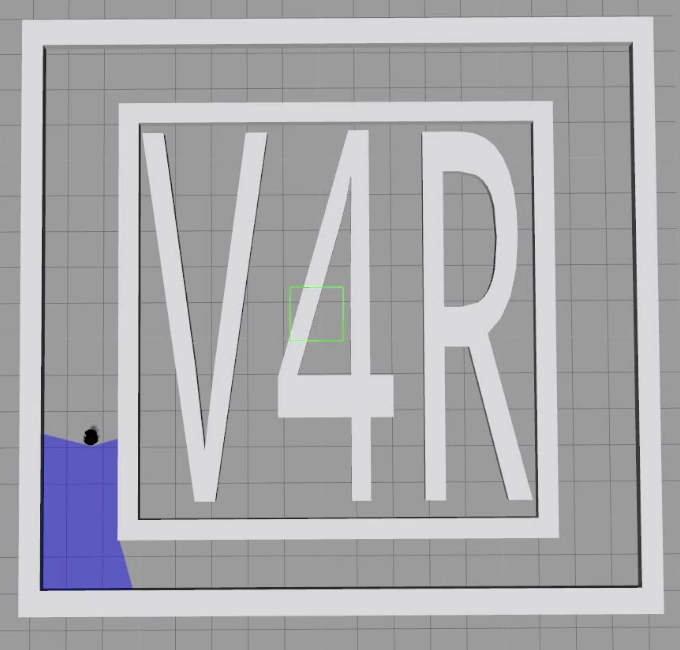
\includegraphics[width=\textwidth]{figures/fig_gazebo_v4r.png}}
       }\\
       \subfloat[]
       {  
           \fbox{
\includegraphics[width=\textwidth]{figures/fig_rviz_v4r.png}}
       }        
       \caption[Simulation environment]{Figure (a) shows the 3D model used for the simulating the robot in the simulation engine. Figure (b) depicts planning information used during the experiments.}
      \label{fig:gazebo_v4r}
   \end{figure}

\section{Results}\label{sec:testresults}
All experiments account for the randomness of the proposed methods by running the algorithm multiple times.
The results are visualized using box-plots. 
The colored box is bounded by the lower quartile and the upper quartile of the data ($25\%$ and $75\%$ of the data). 
The median is indicated by a straight line through the box. 
The upper whisker extending at one end of the box indicate the last data point which lies below the $75\%$ quartile plus $1.5$ times the
inter quartile range (IQR). The lower whisker on the other end indicates the last data point which lies above the $25\%$ quartile minus 1.5 times the IQR. 
Points outside of the whisker range are considered outliers.
As a rule of thumb if the boxes between two measured data sets do not overlap, the difference between those data sets is significant.

Figure~\ref{fig:fig_boxplot} shows a commmon boxplot. 
%\begin{figure}[thpb]
\begin{figure}[thpb]
     \footnotesize
      \centering
      \myfloatalign
      \setlength\fboxsep{0pt}
      \setlength\fboxrule{0.5pt}
       \subfloat[]
       {  
           \fbox{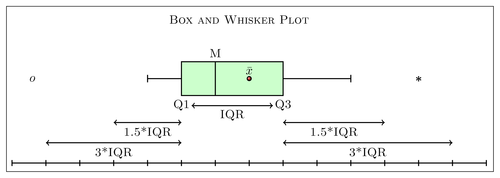
\includegraphics[width=0.75\textwidth]{figures/fig_box-and-whisker-plot.png}}
       }        
       \caption{A classical boxplot diagram.}
      \label{fig:fig_boxplot}
   \end{figure}

\subsection{Influence of trajectory size}
In the first experiment the algorithms were applied to all 60 instances to evaluate a broad spectrum of possible environments. These tests were performed on a 2.4 GHz, Intel Core 2 Duo processor using 4 GB RAM.  
Figure~\ref{fig:fig_allworlds} illustrates the results using 240 trajectories, and using 2400 trajectory samples.
   \begin{figure}[thpb]
        \footnotesize
      \centering
      \def\svgwidth{\textwidth}
      \includesvg{figures/fig_allworlds}
      \caption{This figure shows the results of testing all 60 randomly generated instances. The top figure shows the run time performance for 240 trajectories, and the bottom figure for 2400 trajectories. Compared to brute force search, the Meta-Heuristic algorithms show a significant improvement. }
      \label{fig:fig_allworlds}
   \end{figure}

The results show that all algorithms, including RST, outperform the Brute Force generate-and-test method significantly. 
As expected increasing the number of trajectories greatly favors the Meta-Heuristic algorithms, since they benefit from larger search spaces. 
Notice that ILS and VNS algorithms differ apparently from the RST by exhibiting much smaller variance in their test results, indicating that randomization alone is not enough to achieve very good and stable performance.
Furthermore the VNS exhibit a more stable performance than the ILS methods. 
Comparing the ILS algorithms reveals the connection of the search space size to the size of the neighborhood. 
A small number of trajectories benefits smaller sized neighborhoods, whereas increasing the number of trajectories benefits larger neighborhoods. 

\subsection{Influence of trajectory size by specific instances}
The following tests include the VNSF, VNSB and only one ILS4 algorithm for comparison. 
The algorithms are executed with specific world instances, and repeated 50 times. 
The results in Figure~\ref{fig:fig_special_240} show the application of the algorithm using 240 trajectories. Again the all tested algorithms significantly outperform the Brute Force method. 

\begin{figure}[thb]
   %\myfloatalign
   %\captionsetup[subfigure]{labelformat=empty} 
    %\subfloat[]
    %{  
       \def\svgwidth{\textwidth}
       \includesvg{figures/fig_6_40}
    %}
    \caption[Experiment: Specific instances with 240 trajectories]{The results of 50 consecutively executions with 240 trajectories, on particular instances which differ in number and size of obstacles. The blue line marks the run time for brute force search, which is used as a benchmark.}  
     \label{fig:fig_special_240}
\end{figure}

Increasing the number of trajectories favors the VNS algorithms over the ILS4 algorithm. The results in Figure~\ref{fig:fig_special_960} show the application of the algorithm using 960 trajectories.

\begin{figure}[thb]
   %\myfloatalign
   %\captionsetup[subfigure]{labelformat=empty} 
    %\subfloat[]
    %{  
       \def\svgwidth{\textwidth}
       \includesvg{figures/fig_12_80}
    %}
    \caption[Experiment: Specific instances with 960 trajectories]{The results of 50 consecutively executions with 960 trajectories, on particular instances which differ in number and size of obstacles. The blue line marks the run time for brute force search, which is used as a benchmark.}  
     \label{fig:fig_special_960}
\end{figure}
   
In contrast to the smaller number of trajectories, the results of the ILS4 algorithms shows that a too small environment will quickly degrade to random search if the number of trajectories increases. 
Here the use of a neighborhood structure pays off and the VNS approaches perform evidently better than ILS. 
In addition, the results show that the algorithms perform good independent of number and size of obstacles.

\subsection{Influence of velocity bounds}
The next analysis focus on the influence of the velocity bounds on the performance of the local planning step. 
The trajectory size is fixed to 240 trajectories and the velocity bounds are varied.
Since the previous test has shown that the VNS approach is more promising, the following experiments omit the ILS algorithms.
5 experiments with 50 runs and increasing acceleration windows are conducted.
The test are again performed on different sizes and numbers of obstacles.

In Figure~\ref{fig:fig_vel_big} the results on instances with 1 to 3 obstacle with size 1 meter are presented.  

\begin{figure}[thb]
   \myfloatalign
    \footnotesize
   %\captionsetup[subfigure]{labelformat=empty} 
    \subfloat[]
    {  
       \def\svgwidth{0.75\textwidth}
       \includesvg{figures/vel_comp_b_04_1}
    }\\
    \subfloat[]
    {  
       \def\svgwidth{0.75\textwidth}
       \includesvg{figures/vel_comp_b_19_3}
    }\\
    \subfloat[]
    {  
       \def\svgwidth{0.75\textwidth}
       \includesvg{figures/vel_comp_b_29_3}
    }
    \caption[Experiment: Instances with different velocity bounds (big)]{The results of 50 consecutively executions with 240 trajectories, on instances with 1 (a) and 3 obstacles (b-c) with size 1 meter. The blue line marks the run time for brute force search, which is used as a benchmark.}  
     \label{fig:fig_vel_big}
\end{figure}

 
Figure~\ref{fig:fig_vel_medium} presents the results on instances with 5 obstacles with size 0.5 meter. 

\begin{figure}[thb]
   \myfloatalign
    \footnotesize
   %\captionsetup[subfigure]{labelformat=empty} 
    \subfloat[]
    {  
       \def\svgwidth{0.75\textwidth}
       \includesvg{figures/vel_comp_m_30_5}
    }\\
    \subfloat[]
    {  
       \def\svgwidth{0.75\textwidth}
       \includesvg{figures/vel_comp_m_31_5}
    }\\
    \subfloat[]
    {  
       \def\svgwidth{0.75\textwidth}
       \includesvg{figures/vel_comp_m_44_5}
    }
    \caption[Experiment: Medium obstacle instances with different velocity bounds]{The results of 50 consecutively executions with 240 trajectories, on instances with 5 obstacles with size 0.5 meter. The blue line marks the run time for brute force search, which is used as a benchmark.}  
     \label{fig:fig_vel_medium}
\end{figure}

In Figure~\ref{fig:fig_vel_small} the results on instances with 25 obstacles with size 0.1 meter are presented. 

\begin{figure}[thb]
   \myfloatalign
    \footnotesize
   %\captionsetup[subfigure]{labelformat=empty} 
    \subfloat[]
    {  
       \def\svgwidth{0.75\textwidth}
       \includesvg{figures/vel_comp_s_47_25}
    }\\
    \subfloat[]
    {  
       \def\svgwidth{0.75\textwidth}
       \includesvg{figures/vel_comp_s_53_25}
    }\\
    \subfloat[]
    {  
       \def\svgwidth{0.75\textwidth}
       \includesvg{figures/vel_comp_s_58_25}
    }
    \caption[Experiment: Small obstacle instances with different velocity bounds]{The results of 50 consecutively executions with 240 trajectories, on instances with 25 obstacles with size 0.1 meter. The blue line marks the run time for brute force search, which is used as a benchmark.}  
     \label{fig:fig_vel_small}
\end{figure}

All meta-heuristic algorithms outperform the generate and test method in all instances regardless of the different velocity bounds.
The small instances with many obstacles provide the most difficulties for the proposed methods.
This is increased by using a larger velocity space.
The influence of bigger velocity windows on the performance is not as bad as in the original method.


\subsection{Summary on test result with example planner}
As it is the case for nearly all optimization problems, the No Free Lunch theorems \cite{wolpert1997no} apply also to the local planning domain. 
So it is no surprise that looking at all the results, there is no clear winner among the algorithms. 

Variable Neighborhood search with Tabu List and Best Improvement heuristic seem to yields the best and most stable overall performance, but it is a close call to using this approach with the First Improvement heuristic.

In general the run time of the python implementation is not very efficient compared to tuned C++ implementations. 
Therefore the absolute numbers of the run time evaluations should be handled with care.

\subsection{Simulated environment and robot}
\fxnote{Have the results for the v4r environment using DWA and Trajectory Rollout with and without met-heuristics. Need to make figures.}
